Die Parametrisierung der Templates des Signals und des korrelierten Untergrunds erfolgt durch die $\chi^{2}$-Minimierung.
$\chi^{2}$ gibt dabei ein Maß an, wie gut eine Verteilung an gegebene Daten passt.
Je kleiner $\chi^{2}$ ist, umso besser beschreibt die Verteilung die Daten.
Als freie Parameter für die Parametrisierung werden zwei Skalierungsfaktoren benutzt, einmal ein Skalierungsfaktor für das Template des Signals (SF\textsubscript{Signal}) und einmal ein Skalierungsfaktor für das Template des korrelierten Untergrunds (SF\textsubscript{korr. Untergrund}).
Für $\chi^{2}$ gilt dann:
\begin{align}
\chi^{2} = \sum_{i}\left(\frac{\text{SF}_\text{Signal}\cdot x_{i}+\text{SF}_\text{korr. Untergrund}\cdot y_{i}-z_{i}}{\sqrt{\left(\text{SF}_\text{Signal}\cdot\Delta x_{i}\right)^{2}+\left(\text{SF}_\text{korr. Untergrund}\cdot\Delta y_{i}\right)^{2}+\left(\Delta z\right)^{2}}}\right)^{2}
\label{eq:Chi2}
\end{align}
Hierbei steht $x$ für das Template des Signals, $y$ für das Template des korrelierten Untergrunds und $z$ für die Verteilung der invarianten Masse nach Abzug der unkorrelierten Untergrunds.
Letzteres stammt dabei wieder aus den gemessenen Daten und nicht wie im Abschnitt davor aus einer Simulation.
Der Index $i$, über den summiert wird, läuft über die Intervalle in der invarianten Masse innerhalb des Parametrisierungsbereiches.
Die untere Grenze des Parametrisierungsbereiches wird so gewählt, dass sie außerhalb des Bereiches liegt, wo die Anforderung an den Öffnungswinkel Kombinationsmöglichkeiten ausschließt.
Um diese Werte zu bestimmen wird das Ergebnis der vereinfachten Monte Carlo Simulation benutzt.
Dieses gibt an, ab welchem $m_\text{inv}$ die Wahrscheinlichkeit \textit{Clusterpaare} mit und ohne Anforderung an den Öffnungswinkel zu messen, gleich ist in Abhängigkeit von $p_\text{T}$.
\begin{figure}[t!]
\centering
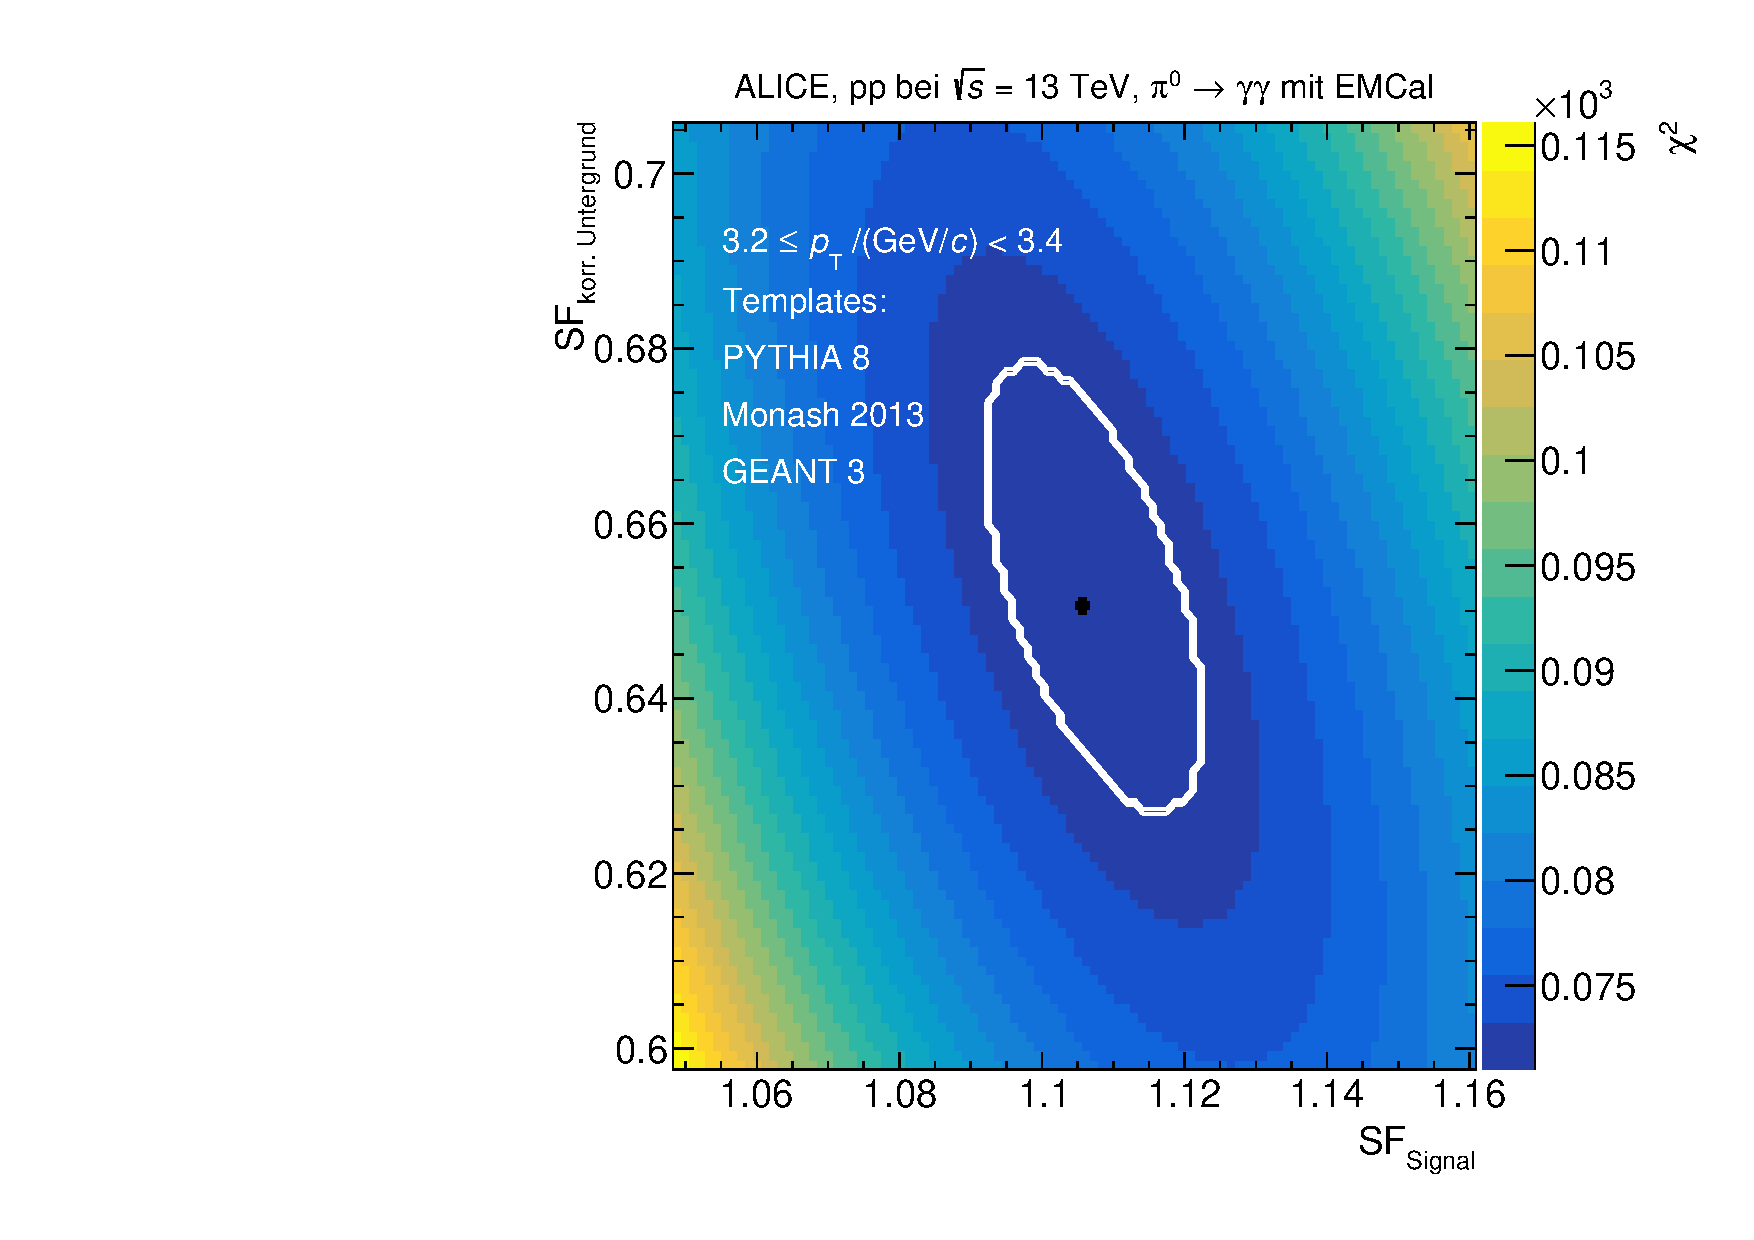
\includegraphics[width=.65\linewidth]{Chi2Map10_Data_2016.pdf}
\caption{$\chi^{2}$ in Abhängigkeit der Skalierungsfaktoren für das Template des Signals und das Template des korrelierten Untergrunds in einem $p_{\text{T}}$-Intervall von $(3\,2 - 3\,4)(\text{GeV}/c)$.
Das schwarze Kreuz in der Mitte liegt auf $\chi^{2}_\text{min}$, während die weiße Kurve um das Minimum die Unsicherheit auf $\chi^{2}_\text{min}$ darstellt.}
\label{fig:Chi2Map}
\end{figure}
\newline
Abbildung \ref{fig:Chi2Map} zeigt die Verteilung von $\chi^{2}$ für unterschiedliche Kombinationen der beiden Skalierungsfaktoren im $p_{\text{T}}$-Intervall $(3\,2 - 3\,4)(\text{GeV}/c)$.
$\chi^{2}_\text{min}$ liegt bei dem schwarzen Kreuz in der Mitte des Bildes.
Die weiße Kurve, die das Minimum umgibt, gibt die Unsicherheit bezüglich der beiden Skalierungsfaktoren an.
Die Werte, die auf der weißen Kurve liegen, werden berechnet durch $\left(\chi^{2}_\text{min}+1\right)$ \cite{book:chi2}.
\newline
Um die Stabilität der Methode zu prüfen wird $\frac{\chi^{2}_\text{min}}{ndf}$ in Abhängigkeit von $p_{\text{T}}$ betrachtet.
Der Nenner ndf steht für die Anzahl der Freiheitsgrade (englisch \textit{\textbf{n}umbers of \textbf{d}egrees of \textbf{f}reedom}).
Die Anzahl an Freiheitsgraden setzt sich dabei aus zwei Teilen zusammen.
Zum einen gilt jeder Datenpunkt in der Verteilung der invarianten Masse, der weder in Daten, noch in einem der Templates den Wert null besitzt und sich innerhalb des Parametrisierungsbereiches befindet, als ein Freiheitsgrad.
Zum anderen wird für jeden freien Parameter die Anzahl an Freiheitsgraden um eins reduziert.
Die Anforderungen an den Öffnungswinkel reduzieren zu höherem $p_{\text{T}}$ hin die Anzahl an Freiheitsgraden zunehmend, weshalb die Normierung von $\chi^{2}_\text{min}$ auf die Anzahl an Freiheitsgraden für einen $p_{\text{T}}$-differenzierten Vergleich notwendig ist.
Außerdem gibt der Wert von $\frac{\chi^{2}_\text{min}}{ndf}$ einen allgemeinen Hinweis auf die Güte der Parametrisierung.
Für $\frac{\chi^{2}_\text{min}}{ndf} = 1$ gilt, dass die Parametrisierung der Templates und die Verteilung der Daten perfekt innerhalb der Unsicherheiten übereinstimmen.
Je größer der Wert von $\frac{\chi^{2}_\text{min}}{ndf}$ , desto weniger gut beschreibt das Template die Verteilung der Daten.
Hingegen bei Werten $\frac{\chi^{2}_\text{min}}{ndf}$ kleiner $1$ gilt, dass die Unsicherheiten in der Verteilung der Daten oder den Templates zu groß sind, für eine sinnvolle Parametrisierung.
\begin{figure}[t!]
\centering
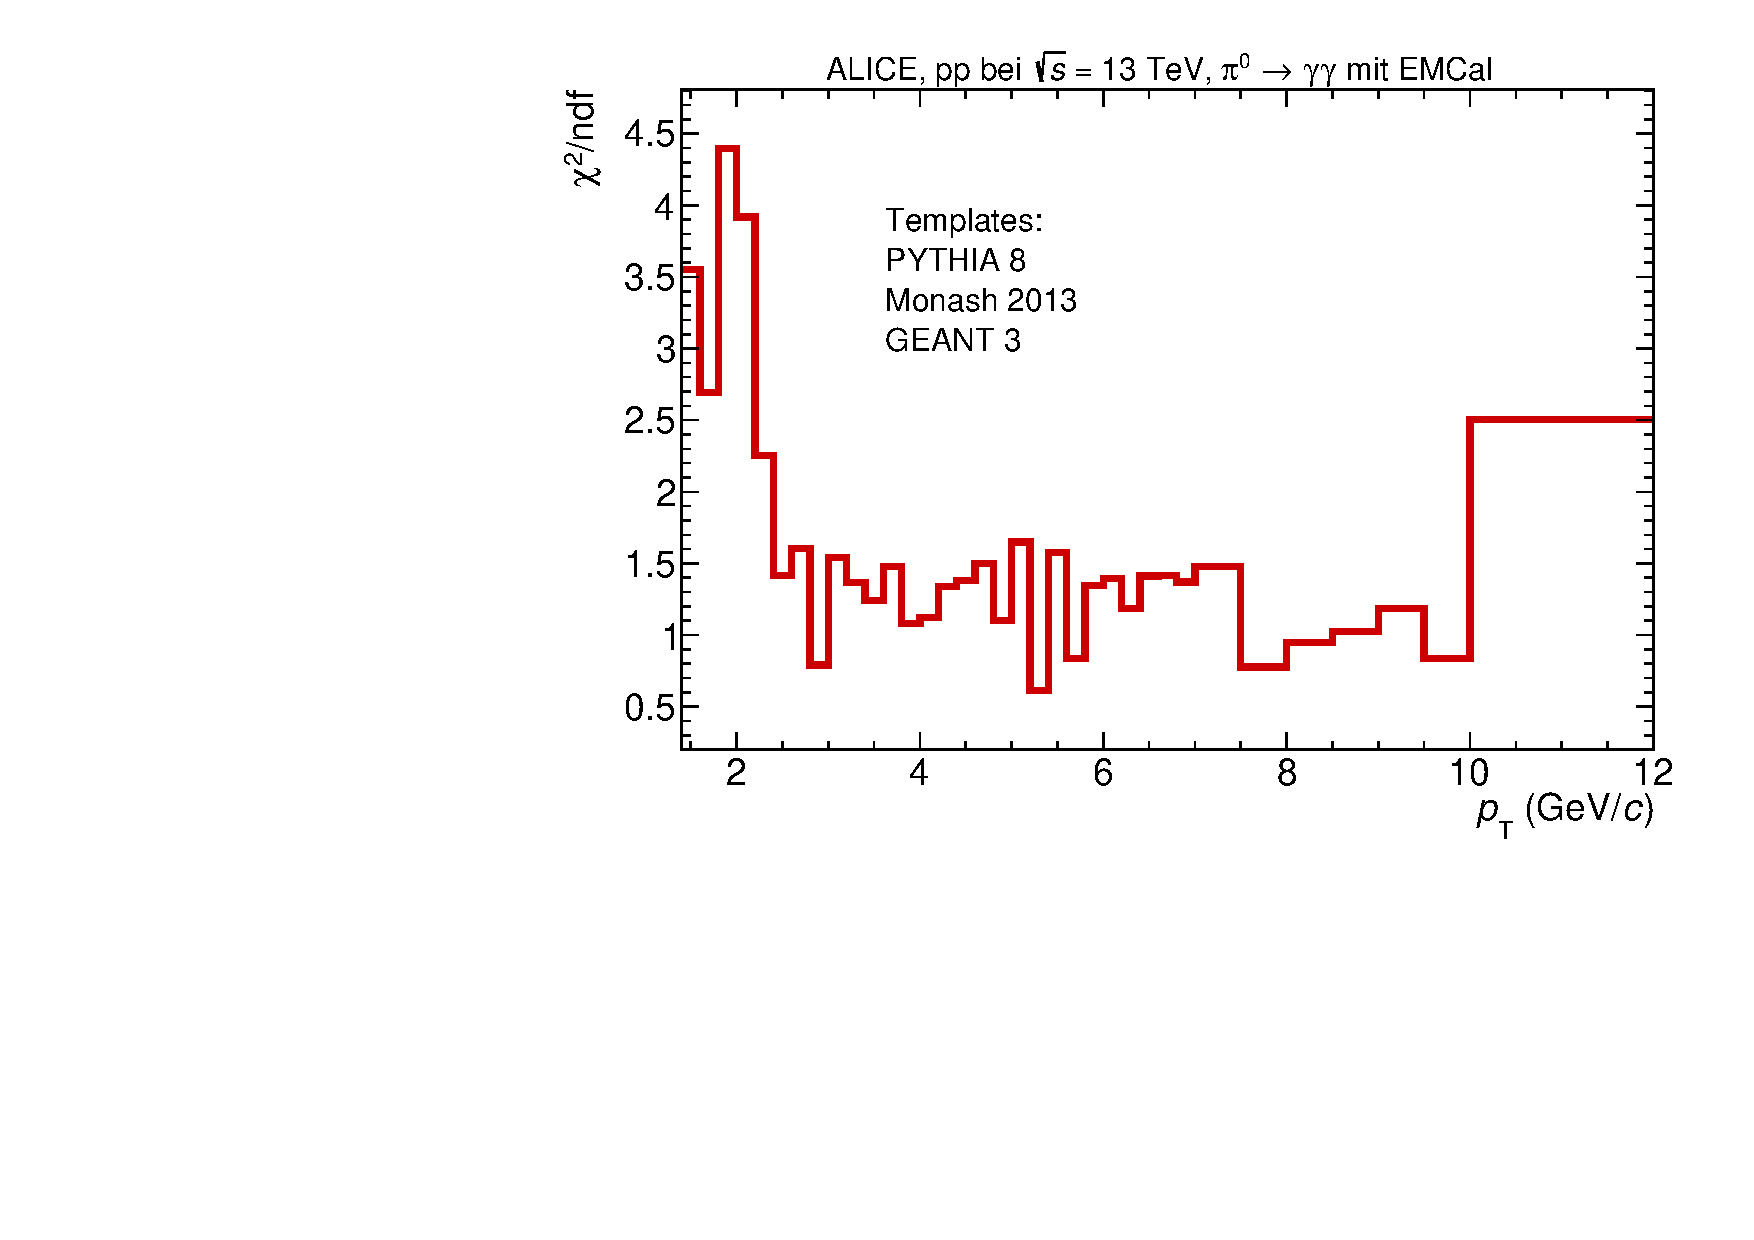
\includegraphics[width=.65\linewidth]{Chi2NoComp_Data_2016.pdf}
\caption{Ergebnis der $\chi^{2}$-Minimierung: $\frac{\chi^{2}_\text{min}}{ndf}$ in Abhängigkeit von $p_{\text{T}}$.
Für $2\,2 \leq p_{\text{T}}/\text{ (GeV}/c) < 10\,0$ liegt der Wert zwischen $0\,6$ und $1\,6$.
Außerhalb dieses $p_\text{T}$-Bereichs weicht $\frac{\chi^{2}_\text{min}}{ndf}$ nach oben ab, bis zu $4\,5$.
}
\label{fig:Chi2pT}
\end{figure}
\newline
Abbildung \ref{fig:Chi2pT} zeigt $\frac{\chi^{2}_\text{min}}{ndf}$ in Ab\-hän\-gig\-keit von $p_{\text{T}}$.
Anfänglich liegt der Wert von $\frac{\chi^{2}_\text{min}}{ndf}$ recht hoch bei fast $4\,5$, bis er bei $p_{\text{T}} >2\,2 \text{ GeV}/c$ schnell sinkt.  
Nach dem Absinken liegt $\frac{\chi^{2}_\text{min}}{ndf}$ um $1\,25$ herum bis $p_{\text{T}} = 7\,5\text{ GeV}/c$.
Ab dort liegt der Wert für $\frac{\chi^{2}_\text{min}}{ndf}$ um $1$ herum, nur für das letzte gezeigte $p_{\text{T}}$-Intervall steigt $\frac{\chi^{2}_\text{min}}{ndf}$ auf einen Wert von $2\,5$.
Insgesamt beschreiben die Templates die Daten also gut.
\begin{figure}[t!]
\centering
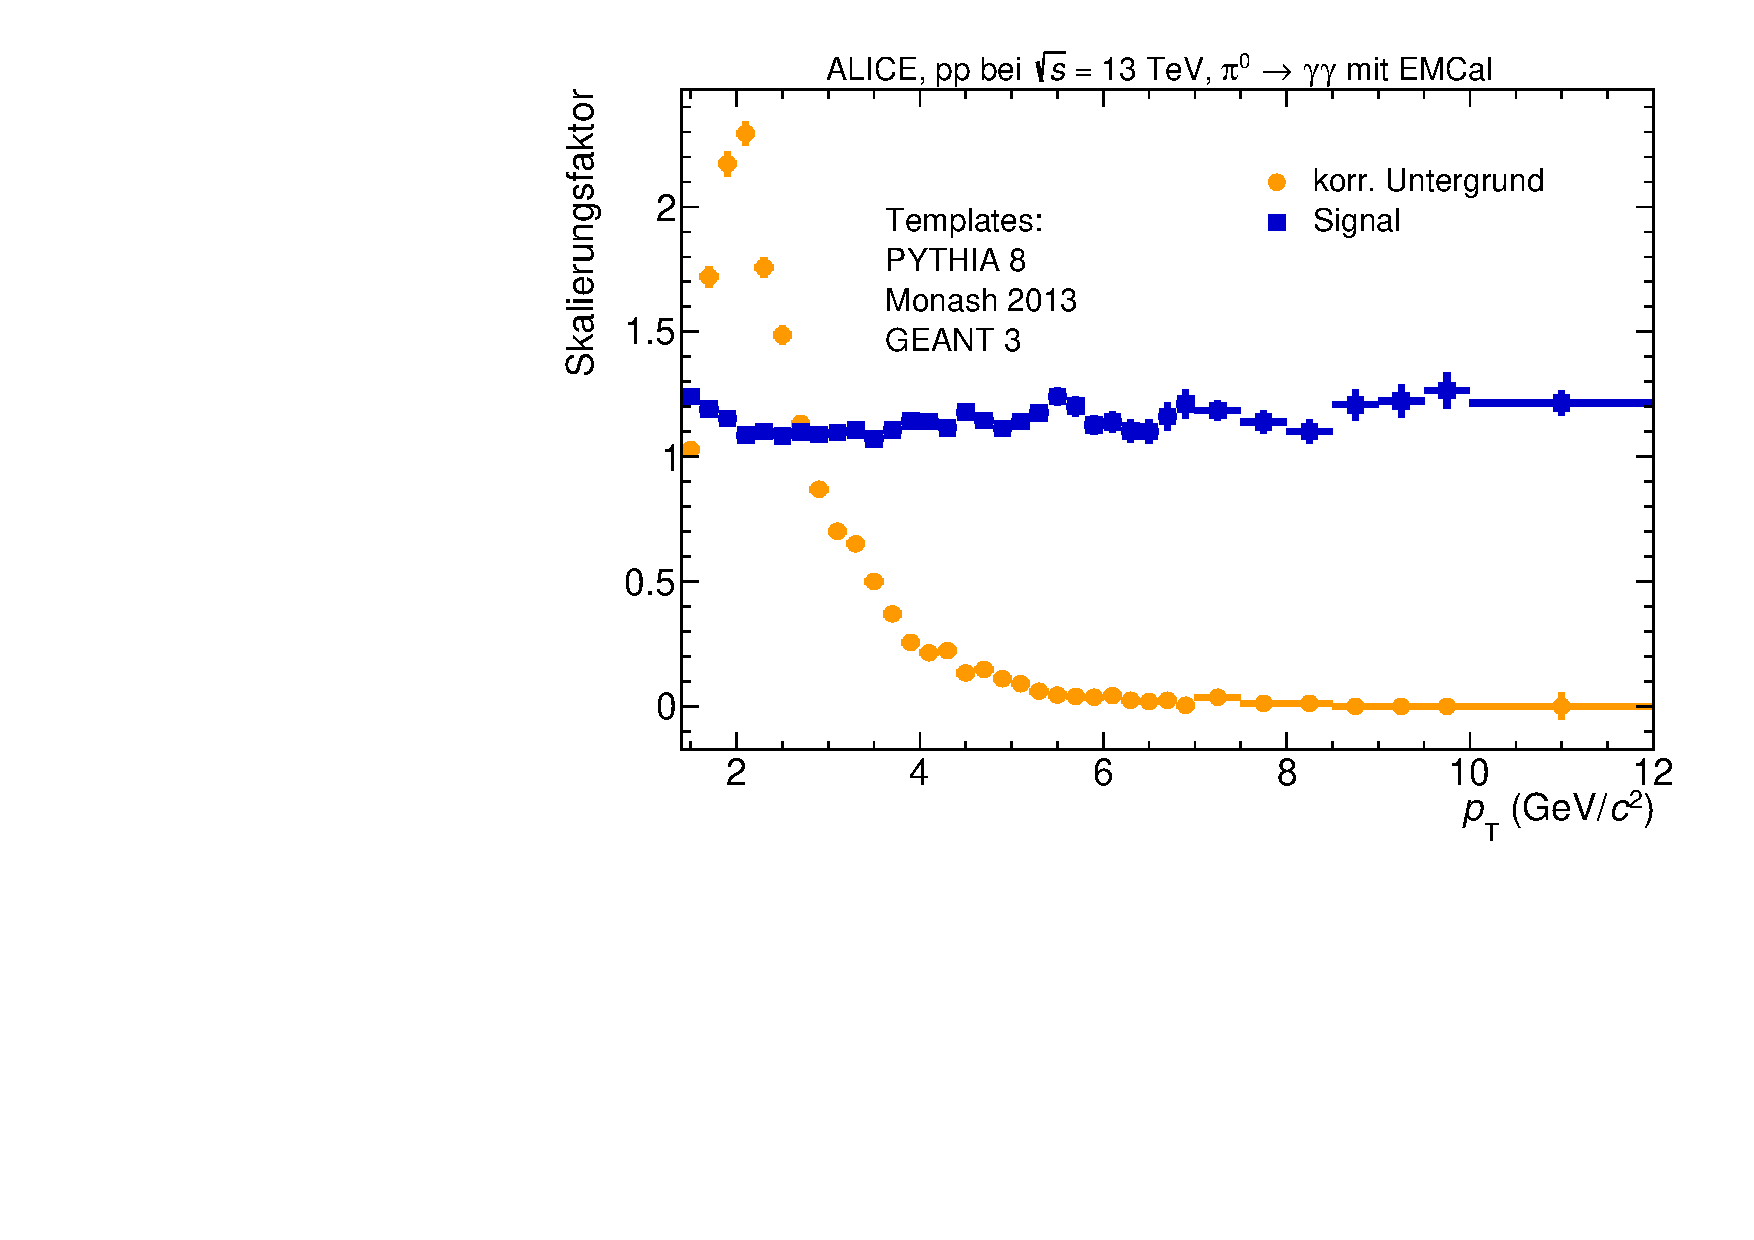
\includegraphics[width=.65\linewidth]{SF_Data_2016.pdf}
\caption{Skalierungsfaktoren der Templates des korrelierten Untergrunds und des Signals in Abhängigkeit von $p_{\text{T}}$.
}
\label{fig:SF}
\end{figure}
\newline
Die Skalierungsfaktoren aus die aus der $\chi^{2}$-Minimierung folgen werden in Abbildung \ref{fig:SF} in Ab\-hän\-gig\-keit von $p_\text{T}$ gezeigt.
Für SF\textsubscript{korr. Untergrund} zeigt sich ein Anstieg bis es sein Maximum bei $1\,8 \leq p_{\text{T}}/(\text{ GeV}/c) < 2\,0$ erreicht.
Vom Maximum aus fällt SF\textsubscript{korr. Untergrund} ab, bis runter zur Null.
Da für alle $p_{\text{T}}$-Intervall das gleiche Template des korrelierten Untergrunds verwendet wird, kann aus dem Verlauf von SF\textsubscript{korr. Untergrund} direkt auf die Menge an korrelierten Untergrund geschlossen werden.
So wird für große $p_{\text{T}}$ kaum bis gar kein korrelierter Untergrund erwartet.
\newline
Die Templates des Signals sind jedoch für jeden $p_{\text{T}}$-Intervall unterschiedlich.
Das annähernd konstante Verhalten von SF\textsubscript{Signal} zeigt entsprechend, dass die Produktionsrate von $\pi^{0}$ in der Simulation gut die Produktionsrate von $\pi^{0}$ im Experiment beschreibt.